\section{�rvores Multidimensionais}

\begin{frame}
	\frametitle{�rvore \textit{K-D}}
	\begin{itemize}
		\item Semelhante � �rvore bin�ria, por�m possibilita a pesquisa por m�ltiplos atributos.
		\item Na �rvore \textit{K-D} os registros s�o definidos por \textit{K} chaves.
		\item A chave que determina s sub-�rvore que ser� acessada, varia a cada n�vel.
		\item No n�vel $L$ a chave $L mod(K+1)$ � utilizada.
	\end{itemize}
\end{frame}

\begin{frame}
	\frametitle{�rvore \textit{K-D}}
	\begin{figure}[h]
	\center
	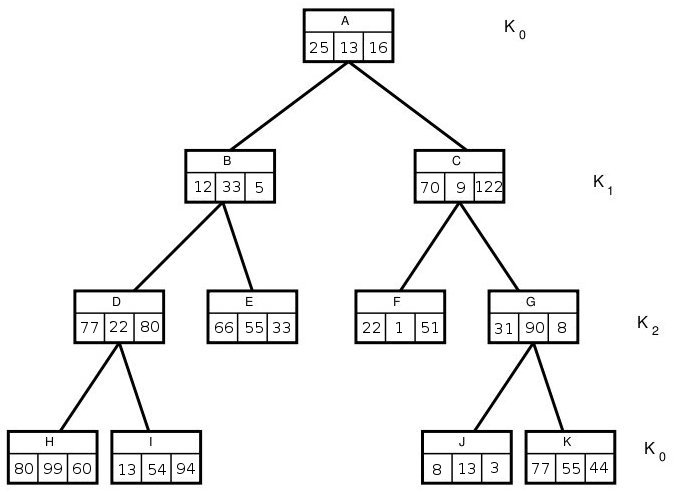
\includegraphics[width=10cm]{../images/kd.jpg}
	\end{figure}
\end{frame}

\begin{frame}
	\frametitle{�rvore \textit{K-D}: Pesquisa}
	\begin{itemize}
		\item Percorre a estrutura usando os crit�rios escolhidos.
		\item Esses crit�rios diferenciam a pesquisa em exata, parcial ou por intervalo.
	\end{itemize}
\end{frame}

\begin{frame}
	\frametitle{�rvore \textit{K-D}: Inser��o}
	\begin{itemize}
		\item Percorre a estrutura usando da pesquisa exata.
		\item Ao encontrar um n� folha, cria um n� com os novos dados e se torna filho do n� folha encontrado.
	\end{itemize}
\end{frame}


